\chapter{Trabajo Relacionado}


\section{Tipos de Relaciones entre Sistemas Autónomos}

El ruteo de los paquetes que transitan por Internet no depende únicamente de la infraestructura física, sino también de las políticas de enrutamiento establecidas entre los Sistemas Autónomos.  Estas políticas están  principalmente influenciadas por las relaciones comerciales entre los ASes~\cite{computing-observed-autonomous-system-relationships-in-the-internet}.\\

Estas relaciones son las que determinan por dónde fluye el tráfico entre los ASes, ya que cada uno define sus políticas basándose en sus necesidades y modelo de negocio. Existen dos tipos principales de relaciones entre los Sistemas Autónomos: customer-to-provider (C2P), donde un cliente paga a un proveedor para acceder a partes del internet que el mismo no alcanza, y peer-to-peer (P2P), donde dos ASes intercambian tráfico destinado a sus respectivos clientes de manera mutua y sin pago de por medio.\\


Gao~\cite{InferringASRelatioships2001} fue la primera en estudiar las relaciones entre los ASes. En su estudio, sentó las bases para abordar su estudio al proponer una forma de representar las relaciones en Internet mediante un grafo parcialmente dirigido (Figura~\ref{fig:tipos-as-rel-chashflow}), donde los nodos representan los Ases y las aristas representan las relaciones entre ellos. En este modelo, las relaciones de customer-to-provider se representan mediante una arista dirigida. Estos acuerdos son más comunes en los bordes del grafo de Internet, donde la topología estaría compuesta  principalmente por ``hojas'', las cuales están principalmente preocupadas por la entrega de su propio tráfico. En contraste, en el núcleo de Internet, la topología consiste en redes densamente interconectadas~\cite{SurveyInterconnectionAgreements}.\\



Conocer las relaciones entre los ASes es de vital importancia, ya que permite entender el comportamiento del tráfico de Internet, detectar posibles ataques y fallos en la red, y optimizar el ruteo de los paquetes. Sin embargo, estas no son de acceso público, por lo que inferir estas relaciones es un problema de gran relevancia en la actualidad. 

A través de las rutas anunciadas mediante BGP, es posible inferir el tipo de relación entre los ASes. \\

La inferencia de estas relaciones ha sido un tema de estudio durante las últimas dos décadas, en las cuales se han propuesto diferentes algoritmos para resolverlo, siendo la mayoría de estos métodos heurísticos   %FIXME: Agregar referencia de los metodos heuristicos InferringASRelatioships2001 \cite{computing-observed-autonomous-system-relationships-in-the-internet} .
utilizando los datos públicos de enrutamiento BGP, como tablas de enrutamiento (RIBs) y anuncios BGP.\\

Gao presentó un primer algoritmo basado en la idea de que el grado de un AS en el grafo suele ser mayor que el de sus clientes, mientras que los ASes peers tienden a tener un grado similar~\cite{InferringASRelatioships2001}. Su método también incorporó el concepto de \textit{valley-free} (VF) en los caminos de enrutamiento.
El concepto de \textit{valley-free} establece que una ruta consistirá en cero o más enlaces C2P, seguido de cero o un 
enlace de peering, y luego cero o más enlaces P2C.

Esta propiedad captura los incentivos económicos que hasta cierto punto determinan el tráfico entre los ASes, ya que un AS no anunciará las rutas aprendidas de un peer o proveedor, eso implicaría el tránsito gratuito de tráfico, lo que aumentaría los costos de infraestructura sin generar beneficios a cambio~\cite{ProbLink}.\\

\begin{figure}[h]
    \centering
    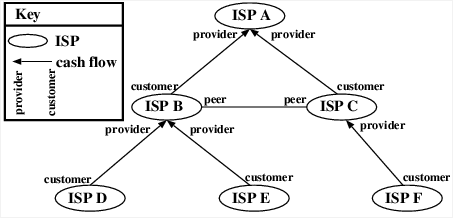
\includegraphics[width=0.7\textwidth]{img/internet/pyramid.png}
    \caption{Tipos de relaciones entre ASes. Fuente https://www.caida.org/catalog/datasets/as-relationships/}
    \label{fig:tipos-as-rel-chashflow}
\end{figure}


Un ejemplo es la Figura \ref{fig:tipos-as-rel-chashflow}, donde el ISP~D le paga al ISP~B para poder acceder al ISP~F, lo que define que tengan una relación del tipo customer-provider. Por otro lado, los ISPs~B y C comparten una relación peer-to-peer, lo que significa que no existe un acuerdo monetario entre ellos, ya que ambos se benefician mutuamente de la conexión. Sin embargo, en este tipo de relación solo se intercambia el tráfico proveniente de sus propios clientes, y no el de sus respectivos proveedores u otros Sistemas Autónomos con los que mantengan relaciones peer-to-peer.\\


\begin{figure}[h]
    \centering
    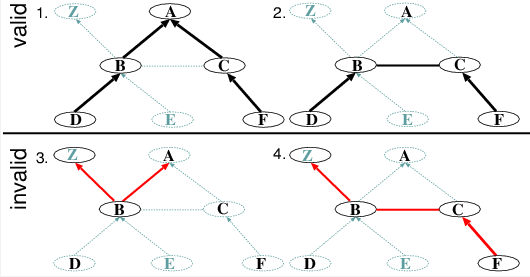
\includegraphics[width=0.7\textwidth]{img/internet/valid-invalid-paths.png}
    \caption{Ejemplos de dos caminos válidos y dos caminos inválidos según el concepto \textit{valley-free}. Fuente https://www.caida.org/catalog/datasets/as-relationships/}    \label{fig:valid-invalid-paths}
\end{figure}


Subramanian et al. \cite{CharacterizingIAS} formularon la tarea como un problema de optimización, definiéndolo como ``the type of relationship (ToR) problem''. Este problema consistía en etiquetar todas las aristas en un grafo de AS para maximizar el número de rutas VF en un conjunto de rutas BGP. Para simplificar el problema, excluyó las relaciones S2S (sibling-to-sibling), que son aquellas que entre dos Ases que pertenecen a un mismo dominio.\\


Se han realizado más estudios que han ido perfeccionando y profundizando en la comprensión del comportamiento de las relaciones entre ASes~\cite{ASRelationshipInferenceValidation,NearDeterministicInference,ProbLink,ComputingTypesRelationshipsBetweenAS,computing-observed-autonomous-system-relationships-in-the-internet}.\\

Luckie et al. \cite{ASRank} introdujeron el algoritmo \textit{AS-Rank} considerando el estado del arte para inferir relaciones C2P y P2P utilizando datos de BGP.
Ellos se basaron en tres supuestos: existe un clique de ASes proveedores de tránsito en la cima de la jerarquía de la topología de Internet, los clientes establecen relaciones con otros ASes con el fin de ser globalmente alcanzables y no existen ciclos de enlaces C2P para que el enrutamiento converja.
Así, introdujeron un nuevo algoritmo para inferir el ``cono de clientes'' de un AS, que es el conjunto de ASes que puede alcanzar utilizando enlaces P2C.\\
 
Por último, Shapira y Shavitt \cite{UnveilingtheTypeRelationshipBetweenAutonomousSystemsUsingDeepLearning} emplearon técnicas de Deep Learning para la tarea de clasificación.
Utilizaron BGP2Vec con el objetivo de crear representaciones de los Sistemas Autónomos y luego pasaron estos \textit{embeddings} 
aprendidos a una Red Neuronal Artificial, la cual se encargó de clasificar los tipos de relaciones entre pares de ASes, 
obteniendo una precisión del 95.2\%. Cabe destacar que el entrenamiento de esta Red Neuronal fue realizado con los datos inferidos del dataset \cite{CAIDAS-relationship}.\\

En nuestro caso desarrollamos esta tarea utilizando Redes Neuronales de Grafos, realizando un experimento similar al de Shapira y Shavitt \cite{UnveilingtheTypeRelationshipBetweenAutonomousSystemsUsingDeepLearning}, pero aplicando GNNs en lugar de una Red Neuronal tradicional. Para ello, primero crearemos un \textit{benchmark} utilizando algunos de los métodos de inferencia de relaciones entre ASes para luego realizar una comparación entre estas técnicas.\\

En el Anexo~\ref{sec:anexo_inferencia_relaciones_as} se presentan métodos que se han desarrollado a lo largo de los años para identificar las relaciones comerciales entre Sistemas Autónomos, junto con su descripción y funcionamiento.\\



\subsection{Importancia de inferir correctamente las relaciones entre Sistemas Autónomos}

Inferir correctamente las relaciones económicas entre Sistemas Autónomos es importante porque estas relaciones influyen directamente en las políticas de exportación de rutas, en la selección de caminos y, en consecuencia, en la estructura observable del enrutamiento interdominio. Una inferencia incorrecta puede llevar a interpretaciones erróneas sobre la jerarquía de Internet, la posición relativa de ciertas redes y la naturaleza de sus interconexiones.\\
% FIXME: Arrgelar el por q es importnat conocerlas para investigacion como route laks o esas cosa sy q no son publicas
Además, conocer estas relaciones permite analizar con mayor precisión la organización económica y topológica de Internet, estudiar fenómenos como la centralidad de ciertos ASes, la presencia de núcleos densamente conectados y la dependencia de redes periféricas respecto de proveedores de tránsito. Esta información también resulta relevante para tareas de simulación, modelado de resiliencia, análisis de seguridad y detección de anomalías, ya que muchas de estas aplicaciones dependen de supuestos sobre cómo fluye el tráfico entre ASes.\\

Por otra parte, dado que las relaciones comerciales no son observables directamente en la mayoría de los casos, su inferencia constituye una tarea fundamental para transformar observaciones parciales del enrutamiento en una representación más interpretable de la estructura de Internet.\\


\subsection{Repositorios de trazas BGP utilizados y sus limitaciones}

Los estudios sobre inferencia de relaciones entre Sistemas Autónomos suelen basarse en repositorios públicos de datos BGP, entre los que destacan \textbf{RouteViews} y \textbf{RIPE RIS}. Estas iniciativas recolectan tablas de enrutamiento (\textit{Routing Information Bases}, RIBs) y mensajes \textit{UPDATE} desde múltiples colectores distribuidos en distintos puntos de Internet. En conjunto con fuentes complementarias como \textbf{CAIDA AS Relationships} y \textbf{PeeringDB}, permiten construir una aproximación de la topología AS-level y enriquecerla con información adicional sobre relaciones y atributos de los ASes.\\

En esta tesis, RouteViews y RIPE RIS se utilizan como fuentes principales de rutas BGP observadas, mientras que CAIDA aporta un conjunto de relaciones utilizado como referencia y PeeringDB provee atributos adicionales de los Sistemas Autónomos. Esta combinación permite construir un grafo de Internet a nivel de AS y estudiar la tarea de inferencia desde una perspectiva comparable con trabajos previos.\\

Sin embargo, estas fuentes no entregan una visión completa de la topología real de Internet. Los datos BGP dependen de la ubicación y cantidad de colectores disponibles, y reflejan únicamente las rutas visibles desde esos puntos de observación. Por ello, la topología inferida a partir de estas fuentes debe entenderse como una aproximación observada y parcial del Internet interdominio.\\

\paragraph{Cobertura limitada de los \textit{vantage points}.}
Una limitación central de los repositorios públicos de rutas BGP es su cobertura incompleta. Cada colector observa únicamente una fracción de las rutas globales, determinada por los \textit{vantage points} o vecinos desde los cuales recibe información. En consecuencia, muchas conexiones entre ASes pueden no aparecer en los datos recolectados, especialmente enlaces de peering privado y relaciones \textit{peer-to-peer}, que suelen ser más difíciles de observar que las relaciones cliente--proveedor. Además, como BGP anuncia principalmente la mejor ruta disponible, enlaces alternativos o de respaldo pueden permanecer ocultos en las RIBs públicas. Por esta razón, el grafo construido a partir de estas fuentes no representa toda la conectividad real de Internet, sino solo la porción visible desde los puntos de observación disponibles.\\


